%%%%%%%%%%%%%%%%%%%%%%%%%%%%%%%%%%%%%%%%%%%%%%%%%%%%%%%%%%%%%%%%%%%%%%%%%%%%%%%%
%2345678901234567890123456789012345678901234567890123456789012345678901234567890
%        1         2         3         4         5         6         7         8

\documentclass[letterpaper, 12 pt, conference]{ieeeconf}  % Comment this line out
                                                          % if you need a4paper
%\documentclass[a4paper, 10pt, conference]{ieeeconf}      % Use this line for a4
                                                          % paper

\IEEEoverridecommandlockouts                              % This command is only
                                                          % needed if you want to
                                                          % use the \thanks command
\overrideIEEEmargins
% See the \addtolength command later in the file to balance the column lengths
% on the last page of the document

\usepackage[utf8]{inputenc}
\usepackage[T1]{fontenc}
\usepackage{graphicx}

% The following packages can be found on http:\\www.ctan.org
%\usepackage{graphics} % for pdf, bitmapped graphics files
%\usepackage{epsfig} % for postscript graphics files
%\usepackage{mathptmx} % assumes new font selection scheme installed
%\usepackage{mathptmx} % assumes new font selection scheme installed
%\usepackage{amsmath} % assumes amsmath package installed
%\usepackage{amssymb}  % assumes amsmath package installed

\title{\LARGE \bf
Machine Translation for Tibetan Buddhist Texts
}

%\author{ \parbox{3 in}{\centering Huibert Kwakernaak*
%         \thanks{*Use the $\backslash$thanks command to put information here}\\
%         Faculty of Electrical Engineering, Mathematics and Computer Science\\
%         University of Twente\\
%         7500 AE Enschede, The Netherlands\\
%         {\tt\small h.kwakernaak@autsubmit.com}}
%         \hspace*{ 0.5 in}
%         \parbox{3 in}{ \centering Pradeep Misra**
%         \thanks{**The footnote marks may be inserted manually}\\
%        Department of Electrical Engineering \\
%         Wright State University\\
%         Dayton, OH 45435, USA\\
%         {\tt\small pmisra@cs.wright.edu}}
%}

\author{ Jacob Atkins$^{1}$, Chris Calloway$^{2}$, Kelsey Namba$^{3}$, Rahul Sehrawat$^{4}$% <-this % stops a space
\thanks{* Supervised by Smara Muresan, Isabelle Zuagg, and Jonathan Reeve}% <-this % stops a space
\thanks{$^{1}$ Jacob Atkins, Columbia '21
        {\tt\small jha2137 at columbia dot edu}}%
        
\thanks{$^{2}$ Chris Calloway, Columbia '21
        {\tt\small cmc2374 at columbia dot edu}}%
        
\thanks{$^{3}$ Kelsey Namba, Columbia '21
        {\tt\small kn2426 at columbia dot edu}}%
        
        
\thanks{$^{3}$ Rahul Sehrawat Columbia '21
        {\tt\small rs3688 at columbia dot edu}}%





}


\begin{document}



\maketitle
\thispagestyle{empty}
\pagestyle{empty}


%%%%%%%%%%%%%%%%%%%%%%%%%%%%%%%%%%%%%%%%%%%%%%%%%%%%%%%%%%%%%%%%%%%%%%%%%%%%%%%%
\begin{abstract}

(Rahul) "PLACEHOLDER PLACEHOLDER PLACEHOLDER PLACEHOLDER PLACEHOLDER PLACEHOLDER PLACEHOLDER PLACEHOLDER PLACEHOLDER PLACEHOLDER PLACEHOLDER
PLACEHOLDER PLACEHOLDER PLACEHOLDER PLACEHOLDER PLACEHOLDER
PLACEHOLDER PLACEHOLDER PLACEHOLDER PLACEHOLDER PLACEHOLDER
PLACEHOLDER PLACEHOLDER PLACEHOLDER PLACEHOLDER PLACEHOLDER
PLACEHOLDER PLACEHOLDER PLACEHOLDER PLACEHOLDER PLACEHOLDER
PLACEHOLDER PLACEHOLDER PLACEHOLDER PLACEHOLDER PLACEHOLDER


\end{abstract}


%%%%%%%%%%%%%%%%%%%%%%%%%%%%%%%%%%%%%%%%%%%%%%%%%%%%%%%%%%%%%%%%%%%%%%%%%%%%%%%%
\section{INTRODUCTION}

Our project aims to increase the accessibility of Tibetan religious texts by training a machine translation model specifically to translate religious Tibetan texts to English. We have trained our models in PyTorch and have leveraged the BART architecture in the HuggingFrance transformers library to make the training and architecture more straightforward. By creating these models, we hope to motivate scholars to study not only these texts but Tibetan as a whole. Currently, while there has been some interest in machine translation for Tibetan-Chinese and vice versa, the same interest has not been reflected in Tibetan-English machine translation. From a deep dive into the open-source Tibetan NLP material, we were unable to find any projects attempting to translate Tibetan-English nor could we find papers specifically discussing Tibetan-English machine translation. By having a readily available set of translated discourses could create an on-ramp for further language uses because increased access could lead to increased interest, especially in the English-speaking community.

\subsection{RELATED WORK}

As a whole, not much work has been done in the area of Machine Translation or even Natural Language Processing as a whole for the Tibetan Language. There are a few papers exist which concern morphological segmentation and POS tagging for the Tibetan language \cite{c3} \cite{c4}. In recent years there has considerable interest in Chinese to Tibetan Machine translation \cite{c1} \cite{c2}. For example, “A Chinese to Tibetan Machine Translation System with Multiple Translating Strategies” discusses an approach of machine translation from Tibetan to Chinese. The paper makes 3 different translations models, Ruled Based MT, Example Based MT, and Statistical Based MT,  and compares the results. Noticeably missing from this is a Neural Network MT. However, Neural Network MT wasn’t prevalent at that time of its authorship. Nonetheless, the paper concludes, given this data (after processing), that the Statistical Based MT (implemented with conditional random fields) is indeed the best performing option. This is perhaps to be expected. However, as is alluded to above it is unknown whether a Neural Network MT would give a better performance here.

The paper “Tibetan-Chinese Neural Machine Translation based on Syllable Segmentation” explores four different methodologies for Tibetan to Chinese machine translation. Chinese and Tibetan are genetically related sharing the same proto-family, the Sino-Tibetan language family. This may mean that the results of this paper may not be fully reflected within our own project. However, there are several important findings that Lai, Zhao, and Bao discovered over the course of their experiment, particularly on the impacts of different models. In 2018, the statistical models were the preferred model type for Tibetan translation tasks, based on the linguistic characteristics of Tibetan. Lai, Zhao, and Bao test whether this is truly the most accurate and efficient model for these tasks by testing Seq2Seq, RNNSearch, Fairseq, and Transformer models against one another. Although each model has its own specific architecture that makes it difficult to normalize settings across all four, the researchers had the same basic parameters (same vocabulary size and training iterations). They also trained each model on two different corpora, one processed based on word segmentation and one processed based on character segmentation (or syllable segmentation). Each model’s performance scores were measured by the BLEU index.

The first model discussed is the Seq2Seq model, or a sequence to sequence model, which is a model that takes in a sequence as input and outputs a sequence as well. The basic idea of a Seq2Seq model is to map the input sequence to the output sequence by taking the input through an LSTM which creates a vector of weighted sums during  the encoding process and returns the words with the highest probability of occurring in the decoder process. The second model tested is the RNNSearch model that adds an attention mechanism, a mechanism that retains the values calculated by the encoding process to train another model which associates the values with output sequences. The new model produces word vectors and then uses these vectors to produce the next word. Although Fairseq models essentially have the same structure as the RNNSearch, where both employ encoder-decoders with attention mechanisms, Fairseq models use CNNs to map the input to the output sequence, which also allows for all the calculations of input sequences to run in parallel. The final model that they tested was the transformer model, which uses the attention mechanism without a CNN or RNN structure. Instead, transformers use a self-attention mechanism that relates all the words in the sentence to one another, where order doesn't matter. Out of these four models, the transformer model trained on the syllable parsed corpus performed the best. For each model tested, they performed substantially better with the syllable parsed corpus than the word parsed corpus. This means that one way we might look to improve our own project’s accuracy is to use a character segmented corpus rather than a word segmented corpus. 

No such papers exist for Tibetan to Enlgish Machine transltions. In fact, to our knowledge this is the first such Tibetan to English Machine translation system developed.  Nonetheless, the findings from the Chinese to Tibetan machine translation have given us a starting point for our investitagion.  



\section{ETHICAL CONSIDERATIONS}

Care must be taken when approaching culturally and spiritually important texts for use in a computational domain. To that end we authors acknowledge our place as outsiders of the Buddhist tradition and outline our ethical approach for translating these texts as said outsiders.

First, we acknowledge that it would be improper to consider our translations as genuine sutras. Regardless of our quantitative results, we authors are not in a qualified position to declare something as an honest translation of a Tibetan Buddhist text. To that end, we have instead given our translations to someone who can give a more qualified opinion of the accuracy of our translation. To this end, we asked a Native Tibetan Speaker who holds a Master's degree in Buddhist theology and philosophy and a current PhD candidate in Tibetan History to  assess our results. This approach to invite someone directly in the Tibetan community to assess our results was inspired by Bird's paper \cite{c7} which suggests including a "human in the loop" as a key step in the process to decolonizing Natural Language Processing research. 

Second, we acknowledge that there are certainly Indo-Tibetan texts that would be inappropriate to translate. These texts, namely the Tantric (esoteric) texts, we understand are meant for a select subset of advanced practitioners and translating these texts for the masses could be spiritually dangerous. Knowing this, we have refrained from including and Tantric texts within our training data. 

Lastly, we acknowledge this is a tool to help bridge the language gap between practitioners both in and out of the Tibetan culture. We authors want to emphasize that this is just a tool. We make no claims that this tool will solve or fix the underlying social injustice issues within Tibetan community and diaspora. While we hope this tool can bring the community closer together and aid in prosperity, we make no claims that it will be able to do so. 

\section{PROCEDURE}


\subsection{Data and Pre-processing}

To train our model, we acquired publicly available English to Tibetan parallel corpora. The non-profit 84000 provided 80 English to Tibetan parallel texts on their website \cite{c8}. All 80 of these texts were expert translations of Indo-Tibetan Buddhist texts. For our model we used all 80 of these provided texts.

Before using 84000's corpora however, we pre-processed the provided data to meet our model's need. The provided files from 84000 were in a .tmx file format, a very standard parallel corpus file format \cite{c9}. 
For our approach, we scraped all 80 .tmx files for both its English and Tibetan contents and placed them line by line into two large .txt files. One .txt file contained the English lines, and the other .txt file contained the Tibetan translation. We made careful assurance that the lines remained in exactly one to one correspondence with their translations. That is, a newline character was used to distinguish two separate lines of translation, but the same line number in each file corresponds to the exact translation provided by 84000. Therefore, the total line numbers in the two .txt files were necessarily the same since one line in one file corresponding to exactly the same line of translated text in the other file. Two such .txt file were made for each of the 80 .tmx files, a Tibetan and an English .txt file for each. After all 160 .txt files were generated, two single large .txt file was generated by concatenating all the Tibetan .txt files and all the English .txt files. These last two .txt files are what was fed into the model.

It was not strictly necessary to separate the creation of the large .txt files into the smaller components. However, giving the limited data we had this method proved useful to see how much individual texts contributed to the model. 




\subsection{Model Design}
We used a 6 layer Transformer model that used a multi headed attention mechanism and a switchout transform. Each layer of the transformer model can be divided into an encoder and decoder layer. The encoding layer consists first of a self attention layer, an attention aspect which focuses on the encoded sentence, and then outputs to a feed forward layer. The multi part of the multi headed attention means that each head will encode the information in parallel and then the results will be concatenated and passed to the decoder. Figure one demonstrates this process.
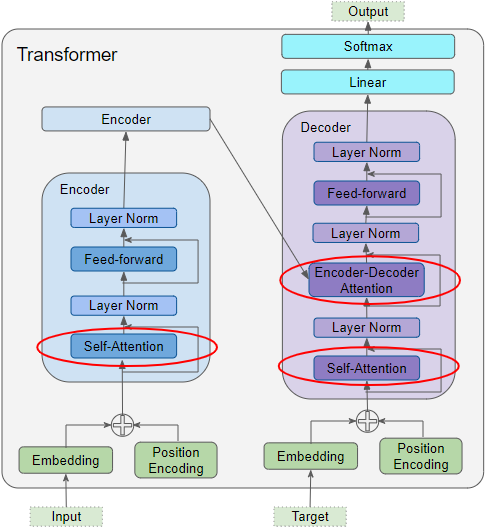
\includegraphics[scale=.4]{Transformer.png}
\caption{\\Figure 1: Overview of a Transformer model}
\\
\par
To prevent overfitting and to augment the data, we added in a switchout transform which will randomly switch out words in the source and target sentence. This also has the added advantage of augmenting the data even further which is especially important for our problem as religious Tibetan has a relatively small corpus, around 30 thousand words. We also attempted to use masking, however we found it to be ineffective. Masking hides tokens from the model by replacing the tokens with a <mask> token. Tibetan tokens are not separated in the same way that latin languages separate their tokens. For example,
\begin{verbatim}
“བྱང་ཆུབ་མངོན་པར་རྫོགས་པར་འཚང་རྒྱ་སྟེ།” 
\end{verbatim}
a line in our test corpus translates to “Having the altruistic intention of excellent bodhicitta.” The Tibetan word is only one token. Therefore, the mask would not help the model learn at all, as the entire sentence would be marked as <mask> and there would not be enough context for our model to discover the meaning. As a result, we did not use any form of masking in our model. Switchout does not create the same problem as their is always a token to take its place. \par
After implementing our transformer model with switchout we tuned hyper parameters to maximize our Transformer model. We manually tuned the following hyperparameters: dropout, label smoothing, rnn size, the number of transformer layers and the number of heads of the attention model. The final configuration used can be found in the appendix. \par
We used four different metrics to evaluate our results: accuracy, predicted score, perplexity and bilingual evaluation understudy (BLEU). The validation accuracy tells us how well we are learning our training data, the predicted score tells us the average log likelihood for each word, the perplexity tells us how well the model predicts the data and the bleu score evaluates the quality of the translation. Together, these metrics provide us with a decent picture of how well our model is performed. 

\section{Results}
\begin{tabular}{ |c| c| c| c| }
 Validation & Ave. Pred. Score & PPL & BLEU \\ 
 40.32\% & -1.69 & 5.41 & 23.01\% \\

\end{tabular}\\

(Jacob)

\section{Discussion}

Considering our use of word segmentation for preprocessing our data (as opposed to character segmentation), our results are comparable with, albeit lower than, Tibetan-Chinese models. Lai, Zhao, and Bao ran several different Tibetan-Chinese models on the same data using two different preprocessing methodologies, character segmentation and word segmentation. Their word segmented Transformer model averaged a higher BLEU score than ours, scoring 38.44\% while our model scored 23.01\%. While this comparison may lead to the conclusion that our model is flawed and irredeemable, only the former is correct. There’s no doubt that our model is underperforming in comparison to other transformer models and hardly makes a correct prediction at all. However, this is most likely due to our difference in preprocessing techniques and the linguistic differences and similarities between English, Chinese, and Tibetan. 

Unlike English but similar to Chinese, Tibetan words are not clearly separated by spaces, rather, characters that represent words are strung together to make a sentence. This makes preprocessing the data and mapping Tibetan words to their English counterparts a difficult task and it makes preprocessing on characters impossible. We trained our model on a parallel corpus of English and Tibetan sentences instead of segmenting each word since preprocessing these sentences to word-to-word mappings would require extensive knowledge of the Tibetan language which our team did not have. On top of this, a Chinese-Tibetan model might perform overall better than a Tibetan-English one since Chinese and Tibetan are part of the same language family, and it is likely that characters may map to one another and the same preprocessing techniques can be used in both languages. Therefore, while comparing our model to Lai, Zhao, and Bao’s model may be helpful to give a general baseline on how other Tibetan translators are performing, it should not be considered where our model must perform.

Another issue with our data that may be remedied in future iterations is the corpora we chose to train and test our model on. Since we trained on sentences in our testing set, it is very possible that the model may have read some of the initial characters and assumed that the entire sentence would be a sentence from our training data that began with the same characters. This may explain why our model overpredicts the sentence “Our blessed one” with such a low perplexity. As stated above, this issue might be remedied if we could preprocess our data so that words mapped to words but since we are limited by our ability to do such, we could consider training our model on a different corpus altogether. Instead of using the translated Buddhist sutras to train our model, we could use a more general Tibetan-English corpus to train our model and then use transfer learning to fine-tune our model to religious texts. However, at this current time, the translated sutras provided by 84000 are some of the only parallel translations available on the internet. 

Perhaps the best way to translate Tibetan to English would be to take another approach to our model design altogether and abandon the tested Transformer model. We could build an Encoder-Decoder structure based on Back Translation which would help deal with the lack of Tibetan-English translations. In this model, we would mix Tibetan and English sentences together to train the model. This would help to increase the size of our training data since it would no longer just be Tibetan sentences. Since this type of model has yet to be tested for Tibetan-English, it's uncertain whether this change could actually improve our translation accuracy and BLEU score, however based on papers written on Back Translation, this design looks promising.


(Kelsey)



\section{Conclusion}


(Rahul)




\section*{ACKNOWLEDGMENT}

The authors would like to thank Palden Gyal for volunteering to read our translated texts. We would also like to thank Smara Muresan, Isabelle Zuagg, and Jonathan Reeve for mentoring this research. Lastly, we would like to thank the 84000 project for providing open source parallel Tibetan corpora. 


(Chris)
\begin{thebibliography}{99}



\bibitem{c1} Cai Z. (2015) A Method for the Chinese-Tibetan Machine Translation System’s Syntactic Analysis. In: Wong W. (eds) Proceedings of the 4th International Conference on Computer Engineering and Networks. Lecture Notes in Electrical Engineering, vol 355. Springer, Cham. 

\bibitem{c2} Liu, H., Zhao, W., Yu, X., & Wu, J. (2016). A Chinese to Tibetan Machine Translation System with Multiple Translating Strategies. Himalayan Linguistics, 15(1).

\bibitem{c3} Hill, Nathan & Meelen, Marieke. (2017). Segmenting and POS tagging Classical Tibetan using a Memory-Based Tagger. Himalayan Linguistics. 16. 10.5070/H916234501. 

\bibitem{c4} Faggionato, Christian  and Meelen, Marieke. (2019). Developing the Old Tibetan Treebank. INCOMA Ltd. Proceedings of the International Conference on Recent Advances in Natural Language Processing (RANLP 2019) 304--312


\bibitem{c5} Orna Almogi, Lena Dankin, Nachum Dershowitz, Lior Wolf. A Hackathon for Classical Tibetan.Journal of Data Mining and Digital Humanities, Episciences.org, 2019, Special Issue on Computer-Aided Processing of Intertextuality in Ancient Languages. hal-01371751v3

\bibitem{c6} Orna Almogi, Lena Dankin, Nachum Dershowitz, Lior Wolf. A Hackathon for Classical Tibetan.Journal of Data Mining and Digital Humanities, Episciences.org, 2019, Special Issue on Computer-Aided Processing of Intertextuality in Ancient Languages. hal-01371751v3


\bibitem{c7} Bird, S. (2020). Decolonising Speech and Language Technology. Proceedings of the 28th International Conference on Computational Linguistics (COLING 2020), 3504–3519.


\bibitem{c8} 84000 Project (2021). What We Do. https://84000.co/about/what-we-do


\bibitem{c9} Coverpages (1997). TMX Format. http://xml.coverpages.org/tmxSpec971212.html




\end{thebibliography}




\end{document}


